\documentclass{article}
\usepackage{graphicx}
\usepackage[margin=1.5cm]{geometry}
\usepackage{csquotes}

\begin{document}

\title{Thursday Reading Assessment: Chapters 13-16 of \textit{Last Place on Earth}}
\author{Prof. Jordan C. Hanson}

\maketitle

\section{Chapter 13 - The Return of the Discovery}

\begin{enumerate}
\item Albert Armitage first ascended the Antarctic Ice Cap, and Robert Falcon Scott returned later to set a record for the ``furthest West.''  Where were they going on these expeditions?  Indicate on the map below the mountains they ascended, now called the Central Trans-Antarctic Mountains.  Indicated on which side of them the ice cap is located.  What were some things that happened to the men on these trips up the mountains?
\begin{figure}[ht]
\centering
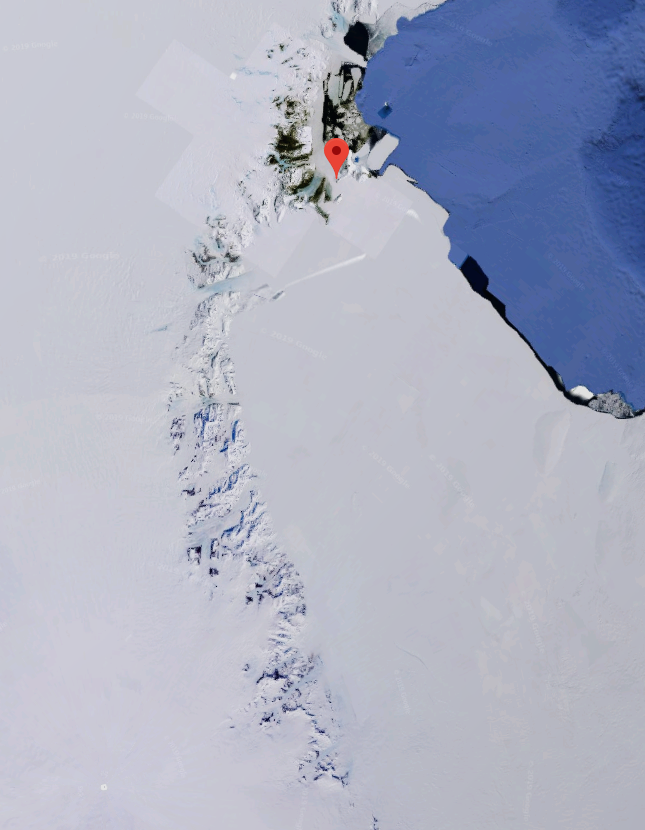
\includegraphics[width=0.25\textwidth]{ice.png}
\caption{\label{fig:ice} The marker indicates Ross Island.  The \textit{Discovery} wintered over in this area.}
\end{figure}
\item Why did the \textit{Discovery} have to be rescued? \\ \vspace{2cm}
\end{enumerate}

\section{Chapter 14 - You Shall Have Fram}

\begin{enumerate}
\item Fridtjof Nansen is quoted in endorsing Roald Amundsen's next adventure:
\begin{displayquote}
(Polar exploration) drives us in to Nature's hidden powers and secrets, down ot the immeasurably little world of the microscopic, and out into the unprobed expanses of the Universe...it gives us no peace until we know this planet on which we live, from the greatest depth of the ocean to the highest layers of the atmosphere.
\end{displayquote}
Describe the general plan of Roald Amundsen to reach the North Pole using the \textit{Fram}, the ship that Nansen had to attempt to reach it. \\ \vspace{3cm}
\end{enumerate}
\section{Chapter 15 - Facing Due South}
\begin{enumerate}
\item Both Dr. Frederick Cook and US Naval Engineer Robert Peary claimed to have reached the North Pole first.  Who was generally accepted to have reached it first by the press and scientific establishment?  Why is navigating using compasses difficult near either pole of the Earth? \\ \vspace{3cm}
\item Who gave Roald Amundsen the idea to \textit{turn South?}  \\ \vspace{2cm}
\end{enumerate}
\section{Chapter 16 - Territorial Waters}
\begin{enumerate}
\item In the period of 1905-1907 both Robert Falcon Scott and Ernest Shackleton were planning trips to the South Pole.  They each considered ``the sledging problem,'' or the problem of \textit{traction} necessary to solve before beginning their journeys.  What device did they attempt to design in order to make getting to the South Pole easier? \\ \vspace{3cm}
\end{enumerate}
\end{document}
